\subsection{Hunyuan Image-to-Video}
% \dq{Tianqi, Weijie, Daquan}
\subsubsection{Pre-training}
\begin{figure}[t]
    \centering
    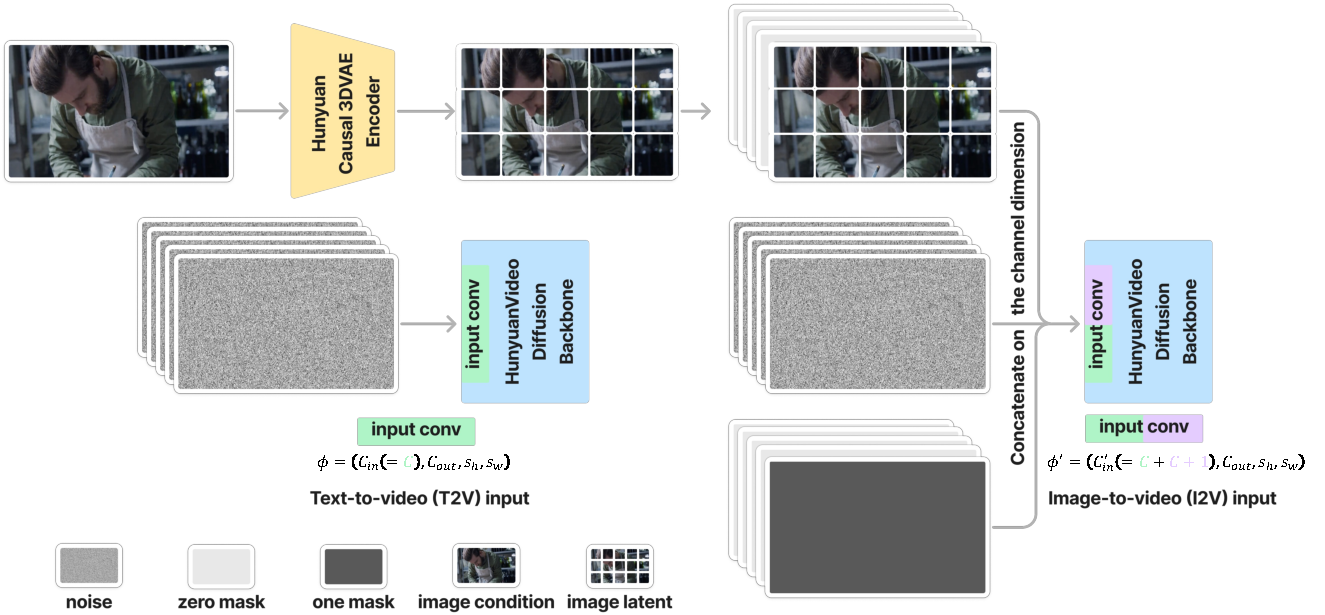
\includegraphics[width=0.9\linewidth]{figures/I2V.pdf}
    \caption{Differences between text-to-video (T2V) model and image-to-video (I2V) model.}
    \label{fig:i2v}
\end{figure}
Image-to-video (I2V) task is a common application in video generation tasks. It usually means that given an image and a caption, the model uses this image as the first frame to generate a video that matches the caption.
Although the naive \nameofmethod{} is a text-to-video (T2V) model, it can be easily extended to an I2V model.
Specifically, as mentioned in Sec. \ref{sec:architecture}, the T2V model's input is a latent $X$ with a shape of $T \times C \times H \times W$, where $T$, $C$, $H$ and $W$ represent the frame, channel, height and width of the compressed video respectively.
Similar to Emu \cite{girdhar2023emu}, in order to introduce image condition $I$, we treat $I$ as the first frame of a video and apply zero-padding to create a $T \times C \times H \times W$ tensor $I_o$, as shown in Fig. \ref{fig:i2v}.
Additionally, we employ a binary mask $m$ with dimensions $T \times 1 \times H \times W$, where the first temporal position is set to 1, and all other positions are set to zero. Then the latent $X$, the tensor $I_o$ and the mask $m$ are concatenated along the channel dimension to form the input for the model.
Note that since the channel of the input tensor has changed from $C$ to $2C+1$, as shown in Fig. \ref{fig:i2v}, we need to adjust the parameters of the first convolutional module of the model from $\phi=(C_{in}(=C), C_{out}, s_h, s_w)$ to $\phi^{\prime}=(C_{in}^{\prime}(=2C+1), C_{out}, s_h, s_w)$, where each component corresponds to the input channel $C_{in}/C_{in}^{\prime}$, output channel $C_{out}$, height of the convolutional kernel $s_h$, and width of the convolutional kernel $s_w$.
In order to retain the representation ability of the T2V model, the first $C$ input channels of $\phi^{\prime}$ are directly copied to $\phi$, and the rest are initialized to zero. We pre-train the I2V model on the same data as T2V model, and the results are shown in Fig. \ref{fig:i2v_result}.
\begin{figure}[t]
    \centering
    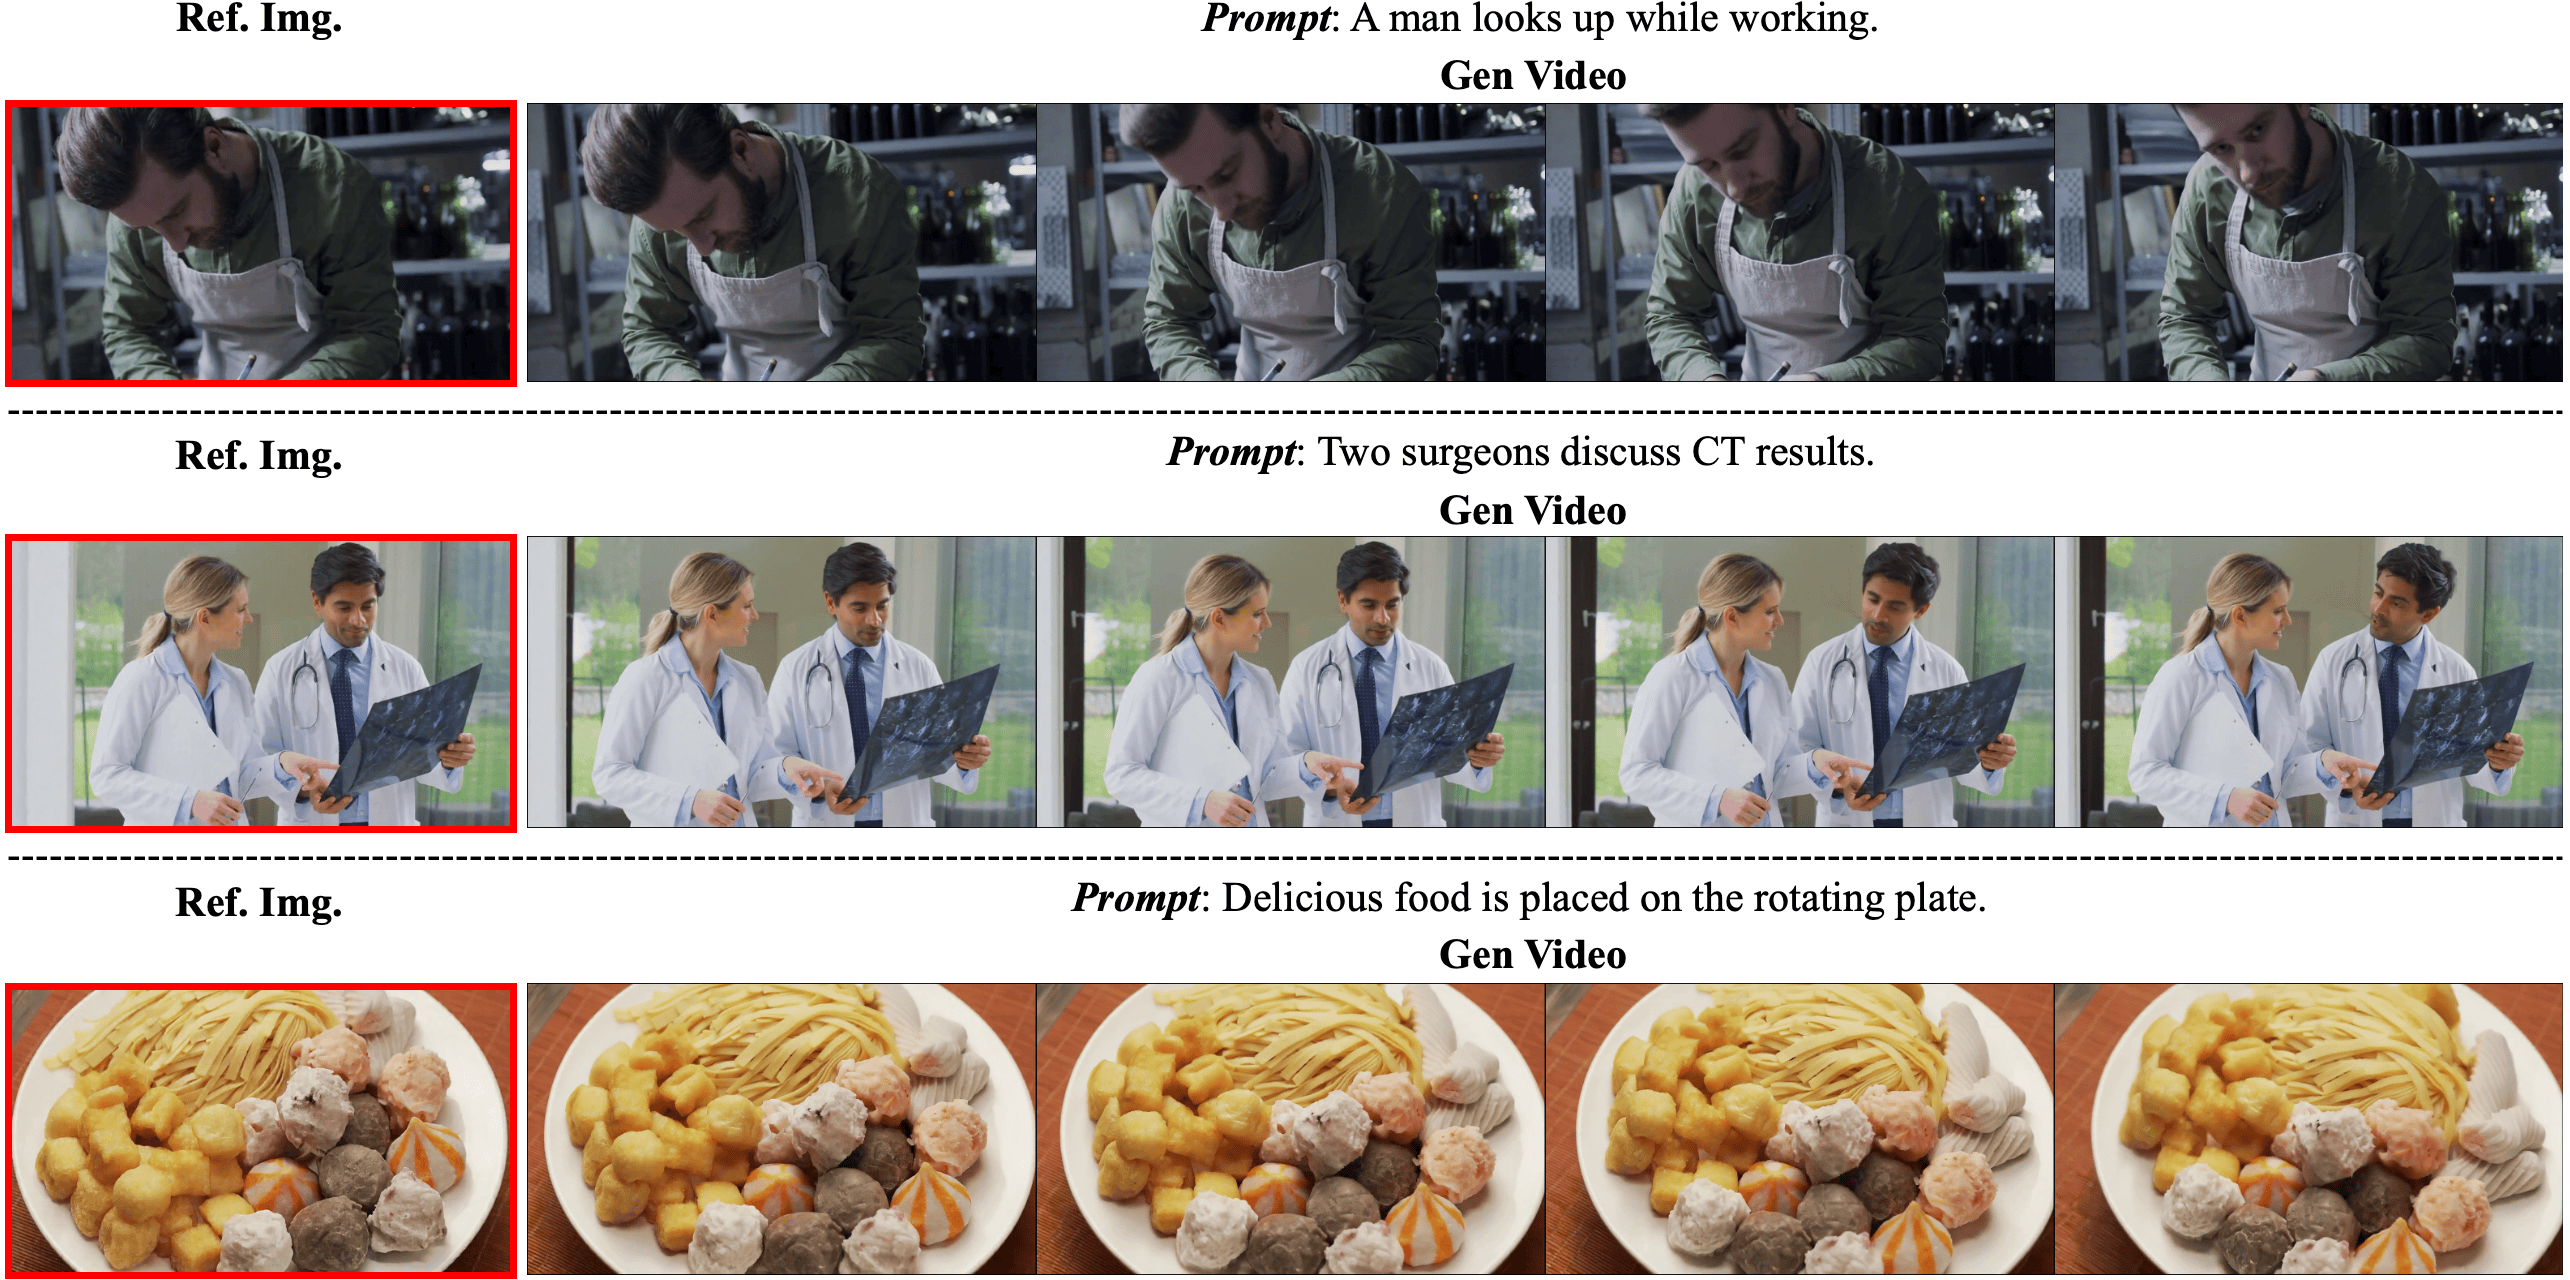
\includegraphics[width=1\linewidth]{figures/i2v_pretraining_result.png}
    \caption{Sample results of the I2V pre-training model.}
    \label{fig:i2v_result}
\end{figure}
